\section{Рабочий проект}

\subsection{Спецификация компонентов и классов программы}

\subsubsection{Модуль main.py}

Модуль предоставляет графический интерфейс для управления базами данных. 

Класс модуля -- MainWindow.

Описание класса MainWindow.
Класс предназначен для управления главным окном приложения и передачи пользовательских команд в обработку. Базовый класс -- Tk, стандартный класс библиотеки Tkinter. Интерфейсы: панель меню, позволяющая выбрать файл базы данных для работы и запустить обработку команды; виджет Treeview, отображающий данные выбранной таблицы; виджет Text, куда пользователь вводит команды. Константы отсутствуют. Внутренние поля представлены в таблице~\ref{table:main_widgets}.

\begin{xltabular}{\textwidth}{|X|X|X|}
	\caption{Внутренние поля класса MainWindow\label{table:main_widgets}} \\
	\hline 
	\centrow Внутреннее поле & 
	\centrow Тип & 
	\centrow Описание \\ 
	\hline 
	\endfirsthead
	
	\caption*{Продолжение таблицы \ref{table:main_widgets}} \\
	\hline 
	\centrow Внутреннее поле & 
	\centrow Тип & 
	\centrow Описание \\ 
	\hline 
	\endhead
	
	selected\_db & Database & Активная база данных, над которой проводятся операции \\ \hline
	main\_menu & Menu & Меню, содержащее пункт для выбора базы данных и пункт для запуска команды \\ \hline
	table\_frame & Frame & Фрейм, содержащий в себе табличный виджет Treeview и скроллбары для его прокрутки \\ \hline
	table & Treeview & Виджет для визуального отображения таблиц и выборки данных \\ \hline
	ysb & Scrollbar & Скроллбар для вертикальной прокрутки таблицы \\ \hline
	xsb & Scrollbar & Скроллбар для горизонтальной прокрутки таблицы \\ \hline
	sql\_field\_frame & Frame & Фрейм, содержащий текстовое поле для ввода команд \\ \hline
	sql\_field & Text & Текстовое поле для ввода команд \\ \hline
\end{xltabular}
Методы класса представлены в таблице~\ref{table:main_method}.
\renewcommand{\arraystretch}{0.8} % уменьшение расстояний до сетки таблицы
\begin{xltabular}{\textwidth}{|>{\hsize=0.85\hsize\raggedright\arraybackslash}X|
		>{\hsize=0.85\hsize\setlength{\baselineskip}{0.7\baselineskip}}X|
		>{\hsize=1.0\hsize}X|
		>{\hsize=1.3\hsize}X|}
	\caption{Методы класса MainWindow\label{table:main_method}}\\
	\hline 
	\centrow \setlength{\baselineskip}{0.7\baselineskip} Название метода & 
	\centrow Параметры метода &
	\centrow Возвращаемое значение & 
	\centrow Назначение метода \\ 
	\hline 
	\endfirsthead
	
	\caption*{Продолжение таблицы \ref{table:main_method}}\\
	\hline 
	\centrow Название метода & 
	\centrow Параметры метода &
	\centrow Возвращаемое значение & 
	\centrow Назначение метода \\ 
	\hline 
	\endhead
	
	\_\_init\_\_ & Не имеет & Не имеет  & Инициализирует графический интерфейс приложения, включая его макет и элементы \\ \hline 
	update\_table & headings -- названия столбцов отображаемой таблицы; contents -- содержимое отображаемой таблицы & Не имеет & Обновляет визуальное отображение таблицы в интерфейсе \\ \hline
	select\_database & Не имеет & Не имеет & Вызывает окно для выбора файла базы данных \\ \hline
	execute\_sql & Не имеет & Не имеет & Вызывает функцию обработки команд из модуля parser.py \\ \hline
	
\end{xltabular}
\renewcommand{\arraystretch}{1.0} % восстановление сетки
\vspace{-\baselineskip}

\subsubsection{Модуль parser.py}

Модуль отвечает за обработку пользовательских команд. Не содержит классов и констант. Методы модуля:
\begin{enumerate}
	\item eval\_node. Обрабатывает логические выражения в условиях where, написанные на синтаксисе Python. Входные данные:
	\begin{itemize}
		\item node (тип ast.Expression) -- условие where;
		\item row (тип dict, значение по умолчанию -- None) -- строка таблицы, из которой нужно взять значения по столбцам.
	\end{itemize}
	
	Возвращаемые данные: результат логического выражения в условии where.
	\item parse\_command. Обрабатывает пользовательские команды. Входные данные:
	\begin{itemize}
		\item command (тип str) -- команда, введённая пользователем в текстовое поле;
		\item db (тип Database) -- движок активной на данный момент базы данных, которому будут передаваться инструкции.
	\end{itemize}
	
	Возвращаемые данные: названия столбцов и содержимое для таблицы в интерфейсе.
\end{enumerate}

\subsubsection{Модуль database.py}

Модуль представляет собой движок, реализующий операции над файлом базы данных.

Класс модуля: Database.

Константы модуля представлены в таблице~\ref{table:db_const}.

\renewcommand{\arraystretch}{0.8}
\begin{xltabular}{\textwidth}{|>{\hsize=1.1\hsize\raggedright\arraybackslash}X|>{\hsize=0.95\hsize\raggedright\arraybackslash}X|>{\hsize=0.95\hsize\raggedright\arraybackslash}X|}
	\caption{Константы модуля database.py\label{table:db_const}} \\
	\hline 
	\centrow Имя константы & 
	\centrow Тип & 
	\centrow Описание \\ 
	\hline 
	\endfirsthead
	
	\caption*{Продолжение таблицы \ref{table:db_const}} \\
	\hline 
	\centrow Имя константы & 
	\centrow Тип & 
	\centrow Описание \\ 
	\hline 
	\endhead
	
	TABLE\_META\_SIZE & int & Размер метаданных таблицы в байтах \\ \hline
	MAX\_TABLE\_COUNT & int & Максимально доступное количество таблиц в базе данных \\ \hline
	MAX\_COLUMN\_COUNT & int & Максимально доступное количество столбцов в таблице \\ \hline
	PAGE\_SIZE & int & Размер одной страницы таблицы в байтах \\ \hline
	DATA\_TYPES & dict & Словарь для сопоставления названий типов данных с их индексом в файле БД \\ \hline
	STRUCT\_TYPES & dict & Словарь для сопоставления типов данных с форматом упаковки значений соответствующего типа данных в бинарный формат \\ \hline
	CHECK\_TYPES & dict & Словарь для проверки корректности типов данных передаваемых для записи в таблицу значений \\ \hline
	DEAD\_END & int & Значение, которое указывается в последней странице таблицы \\ \hline
\end{xltabular}
\renewcommand{\arraystretch}{1.0} % восстановление сетки
\vspace{-\baselineskip}

Описание класса Database. Класс предназначен для выполнения операций над файлом базы данных. Не наследуется от других классов. Интерфейсы -- общедоступные методы \_\_init\_\_, create\_table, insert, select, update, delete, drop\_table. Константы отсутствуют. Внутреннее поле класса -- filepath (тип str), оно хранит путь к файлу базы данных. Методы класса представлены в таблице~\ref{table:db_method}.

\renewcommand{\arraystretch}{0.8} % уменьшение расстояний до сетки таблицы
\begin{xltabular}{\textwidth}{|>{\hsize=0.85\hsize\raggedright\arraybackslash}X|
		>{\hsize=0.85\hsize\setlength{\baselineskip}{0.7\baselineskip}}X|
		>{\hsize=1.0\hsize}X|
		>{\hsize=1.3\hsize}X|}
	\caption{Методы класса Database\label{table:db_method}}\\
	\hline 
	\centrow \setlength{\baselineskip}{0.7\baselineskip} Название метода & 
	\centrow Параметры метода &
	\centrow Возвращаемое значение & 
	\centrow Назначение метода \\ 
	\hline 
	\endfirsthead
	
	\caption*{Продолжение таблицы \ref{table:db_method}}\\
	\hline 
	\centrow Название метода & 
	\centrow Параметры метода &
	\centrow Возвращаемое значение & 
	\centrow Назначение метода \\ 
	\hline 
	\endhead
	
	\_\_init\_\_ & path -- путь к файлу БД & Не имеет  & Инициализирует движок для работы с файлом БД по указанному пути, если такого файла нет, то создаёт его \\ \hline 
	\_allocate\_page & Не имеет & Не имеет & Добавляет пустую страницу в файл БД \\ \hline
	create\_table & table\_name -- имя таблицы; columns -- названия столбцов и их типы данных & Не имеет & Создаёт новую таблицу с указанными именем и столбцами \\ \hline
	insert & table\_name -- имя таблицы; values -- значения, которые будут вставлены в таблицу & Не имеет & Добавляет в страницу новую запись с указанными значениями \\ \hline
	select & table\_name -- имя таблицы; columns -- список столбцов для выборки; where (значение по умолчанию -- lambda row: True) -- условие, по которому будет производиться выборка & Названия и типы данных выбранных столбцов; данные, удовлетворяющие условию & Производит выборку данных в указанных столбцах из строк, удовлетворяющих условию \\ \hline
	update & table\_name -- имя таблицы; updated\_values -- новые значения; where (значение по умолчанию -- lambda row: True) -- условие, по которому будет производиться обновление & Не имеет & Обновляет данные в указанных столбцах в строках, удовлетворяющих условию \\ \hline	
	delete & table\_name -- имя таблицы; where (значение по умолчанию -- lambda row: True) -- условие, по которому будет производиться удаление & Не имеет & Удаляет из таблицы все строки, удовлетворяющие условию \\ \hline
	drop\_table & table\_name -- имя таблицы & Не имеет & Удаляет указанную таблицу из базы данных \\ \hline
	
\end{xltabular}
\renewcommand{\arraystretch}{1.0} % восстановление сетки
\vspace{-\baselineskip}

\subsection{Модульное тестирование разработанной программной системы}

Модульный тест для класса Database из модуля database.py представлен на рисунках~\ref{fig:test_db_1}, ~\ref{fig:test_db_2}, ~\ref{fig:test_db_3}, ~\ref{fig:test_db_4}, ~\ref{fig:dbtestresults}.

\begin{figure}[H]
\begin{lstlisting}[language=Python, breaklines=true]
import unittest
import os
import tempfile
import struct
from database import *

	class TestDatabase(unittest.TestCase):
		def setUp(self):
			self.temp_dir = tempfile.TemporaryDirectory()
			self.db_path = os.path.join(self.temp_dir.name, 'test.db')
			self.db = Database(self.db_path)		
		def tearDown(self):
			self.temp_dir.cleanup()				
		def test_database_initialization(self):
			self.assertTrue(os.path.exists(self.db_path))
			with open(self.db_path, 'rb') as f:
				header = f.read(3)
				table_count, vacant_page = struct.unpack('=BH', header)
				self.assertEqual(table_count, 0)
				self.assertEqual(vacant_page, 0)		
		def test_create_table(self):
			columns = {'id': 'integer', 'name': 'string', 'price': 'float'}
			self.db.create_table('products', columns)
			with open(self.db_path, 'rb') as f:
				table_count = struct.unpack('=B', f.read(1))[0]
				self.assertEqual(table_count, 1)				
				f.seek(3)				
				name, first_page, last_page, rec_size, col_count = struct.unpack('=16sHHHB', f.read(23))
				self.assertEqual(decode_string(name), 'products')
				self.assertEqual(first_page, 0)
				self.assertEqual(last_page, 0)
				self.assertEqual(col_count, 3)				
				col1, type1 = struct.unpack('=16sB', f.read(17))
				col2, type2 = struct.unpack('=16sB', f.read(17))
				col3, type3 = struct.unpack('=16sB', f.read(17))				
				self.assertEqual(decode_string(col1), 'id')
				self.assertEqual(type1, DATA_TYPES['integer'])
				self.assertEqual(decode_string(col2), 'name')
				self.assertEqual(type2, DATA_TYPES['string'])
				self.assertEqual(decode_string(col3), 'price')
				self.assertEqual(type3, DATA_TYPES['float'])
\end{lstlisting}  
\caption{Модульный тест класса Database (1 часть)}
\label{fig:test_db_1}
\end{figure}
	
\begin{figure}[H]
\begin{lstlisting}[language=Python, breaklines=true, firstnumber=42]		
		def test_create_table_errors(self):
			with self.assertRaises(ValueError):
				self.db.create_table('very_long_table_name', {'id': 'integer'})			
			with self.assertRaises(ValueError):
				columns = {f'col{i}': 'integer' for i in range(256)}
				self.db.create_table('too_many_columns', columns)			
			with self.assertRaises(ValueError):
				self.db.create_table('table', {'very_long_column_name': 'integer'})			
			with self.assertRaises(TypeError):
				self.db.create_table('table', {'id': 'unknown_type'})				
		def test_insert_and_select(self):
			self.db.create_table('users', {'id': 'integer', 'name': 'string', 'active': 'integer'})		
			self.db.insert('users', [1, 'Alice', 1])
			self.db.insert('users', [2, 'Bob', 0])
			self.db.insert('users', [3, 'Charlie', 1])			
			columns, data = self.db.select('users', ['*'])
			self.assertEqual(len(data), 3)
			self.assertEqual(data[0]['name'], 'Alice')
			self.assertEqual(data[1]['id'], 2)
			self.assertEqual(data[2]['active'], 1)			
			columns, data = self.db.select('users', ['name', 'active'])
			self.assertEqual(len(data), 3)
			self.assertEqual(set(data[0].keys()), {'name', 'active'})			
			columns, data = self.db.select('users', ['*'], where=lambda row: row['active'] == 1)
			self.assertEqual(len(data), 2)
			self.assertEqual({row['name'] for row in data}, {'Alice', 'Charlie'})			
		def test_insert_errors(self):
			self.db.create_table('test', {'id': 'integer', 'name': 'string'})			
			with self.assertRaises(NameError):
				self.db.insert('nonexistent', [1, 'test'])			
			with self.assertRaises(ValueError):
				self.db.insert('test', [1])			
			with self.assertRaises(TypeError):
				self.db.insert('test', ['not_an_integer', 'test'])
\end{lstlisting}  
\caption{Модульный тест класса Database (2 часть)}
\label{fig:test_db_2}
\end{figure}	
\begin{figure}[H]
\begin{lstlisting}[language=Python, breaklines=true, firstnumber=76]				
		def test_update(self):
			self.db.create_table('products', {'id': 'integer', 'name': 'string', 'price': 'float'})
			self.db.insert('products', [1, 'Apple', 1.99])
			self.db.insert('products', [2, 'Banana', 0.99])
			self.db.insert('products', [3, 'Orange', 2.49])			
			self.db.update('products', {'price': 1.49}, where=lambda row: row['name'] == 'Apple')			
			_, data = self.db.select('products', ['*'])
			apple = next(row for row in data if row['name'] == 'Apple')
			self.assertEqual(round(apple['price'], 2), 1.49)			
			self.db.update('products', {'price': 1.99}, where=lambda row: row['price'] < 2.0)			
			_, data = self.db.select('products', ['*'])
			for row in data:
				if row['price'] < 2.0:
					self.assertEqual(round(row['price'], 2), 1.99)					
		def test_update_errors(self):
			self.db.create_table('test', {'id': 'integer', 'name': 'string'})
			self.db.insert('test', [1, 'test'])			
			with self.assertRaises(NameError):
				self.db.update('nonexistent', {'name': 'new'})			
			with self.assertRaises(NameError):
				self.db.update('test', {'nonexistent': 1})			
			with self.assertRaises(TypeError):
				self.db.update('test', {'id': 'not_an_integer'})				
		def test_delete(self):
			self.db.create_table('orders', {'id': 'integer', 'product': 'string', 'quantity': 'integer'})
			self.db.insert('orders', [1, 'Apple', 5])
			self.db.insert('orders', [2, 'Banana', 3])
			self.db.insert('orders', [3, 'Orange', 2])			
			self.db.delete('orders', where=lambda row: row['id'] == 2)			
			_, data = self.db.select('orders', ['*'])
			self.assertEqual(len(data), 2)
			self.assertEqual({row['id'] for row in data}, {1, 3})			
			self.db.delete('orders')			
			_, data = self.db.select('orders', ['*'])
			self.assertEqual(len(data), 0)
\end{lstlisting}  
\caption{Модульный тест класса Database (3 часть)}
\label{fig:test_db_3}
\end{figure}	
\begin{figure}[H]
\begin{lstlisting}[language=Python, breaklines=true, firstnumber=111]			
		def test_drop_table(self):
			self.db.create_table('temp', {'id': 'integer'})
			self.db.insert('temp', [1])			
			_, data = self.db.select('temp', ['*'])
			self.assertEqual(len(data), 1)			
			self.db.drop_table('temp')			
			with self.assertRaises(NameError):
				self.db.select('temp', ['*'])			
			with open(self.db_path, 'rb') as f:
				table_count = struct.unpack('=B', f.read(1))[0]
				self.assertEqual(table_count, 0)				
		def test_multiple_tables(self):
			self.db.create_table('users', {'id': 'integer', 'name': 'string'})
			self.db.create_table('products', {'id': 'integer', 'name': 'string', 'price': 'float'})			
			self.db.insert('users', [1, 'Alice'])
			self.db.insert('products', [1, 'Apple', 1.99])
			self.db.insert('users', [2, 'Bob'])
			self.db.insert('products', [2, 'Banana', 0.99])			
			_, users = self.db.select('users', ['*'])
			_, products = self.db.select('products', ['*'])			
			self.assertEqual(len(users), 2)
			self.assertEqual(len(products), 2)
			self.assertEqual(users[0]['name'], 'Alice')
			self.assertEqual(products[1]['name'], 'Banana')			
		def test_large_data(self):
			self.db.create_table('large', {'id': 'integer', 'data': 'string'})
			records = 100
			for i in range(records):
				self.db.insert('large', [i, f'Data {i}'])			
			_, data = self.db.select('large', ['*'])
			self.assertEqual(len(data), records)
			self.assertEqual(data[-1]['data'], f'Data {records-1}')			

unittest.main()
\end{lstlisting}  
\caption{Модульный тест класса Database (4 часть)}
\label{fig:test_db_4}
\end{figure}

Результат тестирования:
\begin{figure}[H]
	\centering
	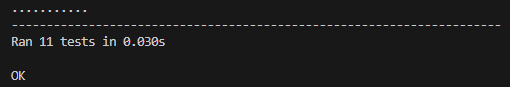
\includegraphics[width=0.7\linewidth]{images/dbtestresults}
	\caption{Результат тестирования класса UNet}
	\label{fig:dbtestresults}
\end{figure}

Модульный тест для функций eval\_node и parse\_command из модуля parser.py представлен на рисунках~\ref{fig:test_parser_1}, ~\ref{fig:test_parser_2}, ~\ref{fig:test_parser_3}, ~\ref{fig:test_parser_4}, ~\ref{fig:test_parser_results}.

\begin{figure}[H]
	\begin{lstlisting}[language=Python, breaklines=true]			
		import unittest
		import ast
		import os
		from database import Database
		from parser import *
		
		TEST_DB_PATH = 'test_db.db'
		
		class TestEvalNode(unittest.TestCase):
		def test_constant(self):
		node = ast.parse("42", mode='eval')
		self.assertEqual(eval_node(node), 42)        
		node = ast.parse("3.14", mode='eval')
		self.assertEqual(eval_node(node), 3.14)        
		node = ast.parse("'hello'", mode='eval')
		self.assertEqual(eval_node(node), 'hello')        
		node = ast.parse("True", mode='eval')
		self.assertEqual(eval_node(node), True)
		def test_name(self):
		row = {'x': 10, 'y': 20}
		node = ast.parse("x", mode='eval')
		self.assertEqual(eval_node(node, row), 10)        
		node = ast.parse("y", mode='eval')
		self.assertEqual(eval_node(node, row), 20)
		def test_dict(self):
		node = ast.parse("{'a': 1, 'b': 2}", mode='eval')
		self.assertEqual(eval_node(node), {'a': 1, 'b': 2})        
		row = {'x': 10}
		node = ast.parse("{'a': x, 'b': x+5}", mode='eval')
		self.assertEqual(eval_node(node, row), {'a': 10, 'b': 15})
		def test_binop(self):
		node = ast.parse("2 + 3", mode='eval')
		self.assertEqual(eval_node(node), 5)        
		node = ast.parse("5 - 2", mode='eval')
		self.assertEqual(eval_node(node), 3)        
		node = ast.parse("2 * 3", mode='eval')
		self.assertEqual(eval_node(node), 6)        
		node = ast.parse("6 / 2", mode='eval')
		self.assertEqual(eval_node(node), 3)        
		node = ast.parse("7 // 2", mode='eval')
		self.assertEqual(eval_node(node), 3)        
		node = ast.parse("7 % 2", mode='eval')
		self.assertEqual(eval_node(node), 1)        
		node = ast.parse("2 ** 3", mode='eval')
		self.assertEqual(eval_node(node), 8)		
	\end{lstlisting}  
	\caption{Модульный тест parser.py (1 часть)}
	\label{fig:test_parser_1}
\end{figure}

\begin{figure}[H]
	\begin{lstlisting}[language=Python, breaklines=true]
		def test_compare(self):
			node = ast.parse("5 > 3", mode='eval')
			self.assertEqual(eval_node(node), True)        
			node = ast.parse("5 >= 5", mode='eval')
			self.assertEqual(eval_node(node), True)        
			node = ast.parse("3 < 5", mode='eval')
			self.assertEqual(eval_node(node), True)        
			node = ast.parse("5 <= 5", mode='eval')
			self.assertEqual(eval_node(node), True)        
			node = ast.parse("5 == 5", mode='eval')
			self.assertEqual(eval_node(node), True)        
			node = ast.parse("5 != 3", mode='eval')
			self.assertEqual(eval_node(node), True)
		def test_boolop(self):
			node = ast.parse("True and False", mode='eval')
			self.assertEqual(eval_node(node), False)        
			node = ast.parse("True or False", mode='eval')
			self.assertEqual(eval_node(node), True)        
			node = ast.parse("True and True and False", mode='eval')
			self.assertEqual(eval_node(node), False)        
			node = ast.parse("False or False or True", mode='eval')
			self.assertEqual(eval_node(node), True)
		def test_unaryop(self):
			node = ast.parse("-5", mode='eval')
			self.assertEqual(eval_node(node), -5)        
			node = ast.parse("not True", mode='eval')
			self.assertEqual(eval_node(node), False)        
			node = ast.parse("not False", mode='eval')
			self.assertEqual(eval_node(node), True)
		def test_unsupported_node(self):
			node = ast.parse("lambda x: x+1", mode='eval')
			with self.assertRaises(ValueError):
			eval_node(node)
	class TestParseCommand(unittest.TestCase):
		@classmethod
		def setUpClass(cls):
			if os.path.exists(TEST_DB_PATH):
				os.remove(TEST_DB_PATH)
			cls.db = Database(TEST_DB_PATH)	
		@classmethod
		def tearDownClass(cls):
			if os.path.exists(TEST_DB_PATH):
				os.remove(TEST_DB_PATH)
		def setUp(self):
			if os.path.exists(TEST_DB_PATH):
				os.remove(TEST_DB_PATH)
			self.db = Database(TEST_DB_PATH)
	\end{lstlisting}  
\caption{Модульный тест parser.py (2 часть)}
\label{fig:test_parser_2}
\end{figure}
\begin{figure}[H]
\begin{lstlisting}[language=Python, breaklines=true]	
	def test_empty_command(self):
		with self.assertRaises(CommandError):
			parse_command("", self.db)
	def test_create_table(self):
		result = parse_command("create table users id integer name string age integer", self.db)
		self.assertEqual(len(result[1]), 0)            
		with self.assertRaises(CommandError):
			parse_command("create table", self.db)            
		with self.assertRaises(CommandError):
			parse_command("create table users", self.db)            
		with self.assertRaises(CommandError):
			parse_command("create table users id", self.db)
	def test_create_database(self):
		name = 'test_new_db'
		temp_db_path = f'databases/{name}.db'
		try:
			result = parse_command(f"create database {name}", self.db)
			self.assertIsInstance(result, Database)
			self.assertTrue(os.path.exists(temp_db_path))
		finally:
			if os.path.exists(temp_db_path):
				os.remove(temp_db_path)
	def test_insert(self):
		parse_command("create table users id integer name string age integer", self.db)
		result = parse_command("insert into users values 1 'Alice' 25", self.db)
		self.assertEqual(len(result[1]), 1)
		self.assertEqual(result[1][0], {'id': 1, 'name': 'Alice', 'age': 25})            
		with self.assertRaises(CommandError):
			parse_command("insert users values 1 'Alice'", self.db)            
		with self.assertRaises(CommandError):
			parse_command("insert into users 1 'Alice' 25", self.db)
	def test_select(self):
		parse_command("create table users id integer name string age integer", self.db)
		parse_command("insert into users values 1 'Alice' 25", self.db)
		parse_command("insert into users values 2 'Bob' 30", self.db)        
		result = parse_command("select * from users", self.db)
		self.assertEqual(len(result[1]), 2)        
		result = parse_command("select name age from users", self.db)
		self.assertEqual(len(result[1]), 2)
		self.assertEqual(list(result[1][0].keys()), ['name', 'age'])  
		result = parse_command("select * from users where age > 25", self.db)
		self.assertEqual(len(result[1]), 1)
		self.assertEqual(result[1][0]['name'], 'Bob')            
		with self.assertRaises(CommandError):
			parse_command("select from users", self.db)            
		with self.assertRaises(CommandError):
			parse_command("select * users", self.db)
\end{lstlisting}  
\caption{Модульный тест parser.py (3 часть)}
\label{fig:test_parser_3}
\end{figure}
\begin{figure}[H]
\begin{lstlisting}[language=Python, breaklines=true]		
	def test_update(self):
		parse_command("create table users id integer name string age integer", self.db)
		parse_command("insert into users values 1 'Alice' 25", self.db)
		parse_command("insert into users values 2 'Bob' 30", self.db)        
		result = parse_command("update users set name 'Rachel' age 26 where id == 1", self.db)
		self.assertEqual(len(result[1]), 2)
		updated = next(row for row in result[1] if row['id'] == 1)
		self.assertEqual(updated['name'], 'Rachel')
		self.assertEqual(updated['age'], 26)            
		with self.assertRaises(CommandError):
			parse_command("update users name 'Alice'", self.db)            
		with self.assertRaises(CommandError):
			parse_command("update users set name where id == 1", self.db)
	def test_delete(self):
		parse_command("create table users id integer name string age integer", self.db)
		parse_command("insert into users values 1 'Alice' 25", self.db)
		parse_command("insert into users values 2 'Bob' 30", self.db)        
		result = parse_command("delete from users where age < 30", self.db)
		self.assertEqual(len(result[1]), 1)
		self.assertEqual(result[1][0]['name'], 'Bob')            
		with self.assertRaises(CommandError):
			parse_command("delete users where age < 30", self.db)        
	def test_drop_table(self):
		parse_command("create table users id integer name string age integer", self.db)
		parse_command("insert into users values 1 'Alice' 25", self.db)        
		result = parse_command("drop table users", self.db)
		self.assertEqual(result, ([], [{}]))        
		with self.assertRaises(NameError):
			parse_command("select * from users", self.db)        
		with self.assertRaises(CommandError):
			parse_command("drop users", self.db)            
		with self.assertRaises(CommandError):
			parse_command("drop table", self.db)
	def test_unknown_command(self):
		with self.assertRaises(CommandError):
			parse_command("unknown command", self.db)	

unittest.main()
\end{lstlisting}  
\caption{Модульный тест parser.py (4 часть)}
\label{fig:test_parser_4}
\end{figure}

Результат тестирования:
\begin{figure}[H]
	\centering
	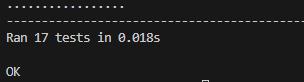
\includegraphics[width=0.7\linewidth]{images/test_parser_results}
	\caption{Результат тестирования функций модуля parser.py}
	\label{fig:test_parser_results}
\end{figure}

\subsection{Системное тестирование разработанной программной системы}

Для проведения системного тестирования был использован файл базы данных, содержащий таблицу с сотней записей.

На рисунке~\ref{fig:dbms_window} представлено главное окно СУБД.
\begin{figure}[H]
	\centering
	\includegraphics[width=0.7\linewidth]{"images/окно субд"}
	\caption{Главное окно программы}
	\label{fig:dbms_window}
\end{figure}

На рисунке~\ref{fig:select} представлено окно выбора файла после нажатия на пункт меню <<Выбрать БД>>.
\begin{figure}[H]
	\centering
	\includegraphics[width=0.7\linewidth]{"images/выбор файла"}
	\caption{Окно выбора файла}
	\label{fig:select}
\end{figure}

На рисунке~\ref{fig:select_sql} представлен результат выборки данных из таблицы.
\begin{figure}[H]
	\centering
	\includegraphics[width=0.7\linewidth]{"images/выборка"}
	\caption{Результат выборки}
	\label{fig:select_sql}
\end{figure}

На рисунке~\ref{fig:error} представлено сообщение об ошибке при неправильно введённой команде.
\begin{figure}[H]
	\centering
	\includegraphics[width=0.7\linewidth]{"images/ошибка"}
	\caption{Ошибка в команде}
	\label{fig:error}
\end{figure}

На рисунке~\ref{fig:error_table} представлено сообщение об ошибке при попытке обращения к несуществующей таблице.
\begin{figure}[H]
	\centering
	\includegraphics[width=0.7\linewidth]{"images/ошибка таблица"}
	\caption{Обращение к несуществующей таблице}
	\label{fig:error_table}
\end{figure}

На рисунке~\ref{fig:new_db} показана информация о файле новой базы данных, созданной после ввода команды create database new\_database.
\begin{figure}[H]
	\centering
	\includegraphics[width=0.7\linewidth]{"images/новая бд"}
	\caption{Обращение к несуществующей таблице}
	\label{fig:new_db}
\end{figure}

\subsection{Сборка программной системы}

Программные компоненты представляют собой файлы исходных кодов программной системы.

Для сборки и компиляции программной системы использовалась библиотека Pyinstaller, позволяющая упаковать все необходимые файлы в один исполняемый файл формата .exe. Данный файл может быть запущен без предварительной установки.

Интерпретация исходных кодов на языке Python выполняется встроенным в исполняемый файл интерпретатором языка и не требует отдельной установки интерпретатора и библиотек на целевую систему.

Все программные компоненты собраны в один исполняемый файл, готовый к запуску в среде Windows.